\chapter{Analisis}
\label{chap:analisis}

Bab ini menjelaskan mengenai analisis perangkat lunak sejenis, analisis metode penyimpanan informasi login, analisis metode rekam dan kirim informasi login, analisis metode deteksi \textit{captive portal} , serta analisis perangkat lunak.



\section{Analisis Perangkat Lunak Sejenis}
\label{sec:perangkat_lunak_sejenis}

Perangkat lunak sejenis pada Windows belum dapat ditemukan pada saat penelitian ini dilakukan. Oleh karena itu, perangkat lunak atau aplikasi sejenis yang dianalisis adalah aplikasi yang diciptakan untuk sistem operasi Android. Aplikasi tersebut bernama \textit{WiFi Web Login}\footnote{https://play.google.com/store/apps/details?id=co.uk.syslynx.wifiwebloginapp}.

\subsubsection{Tampilan \textit{WiFi Web Login}}
\label{subsubsec:tampilan_wifi_web_login}

\begin{figure}[h]
    \centering
    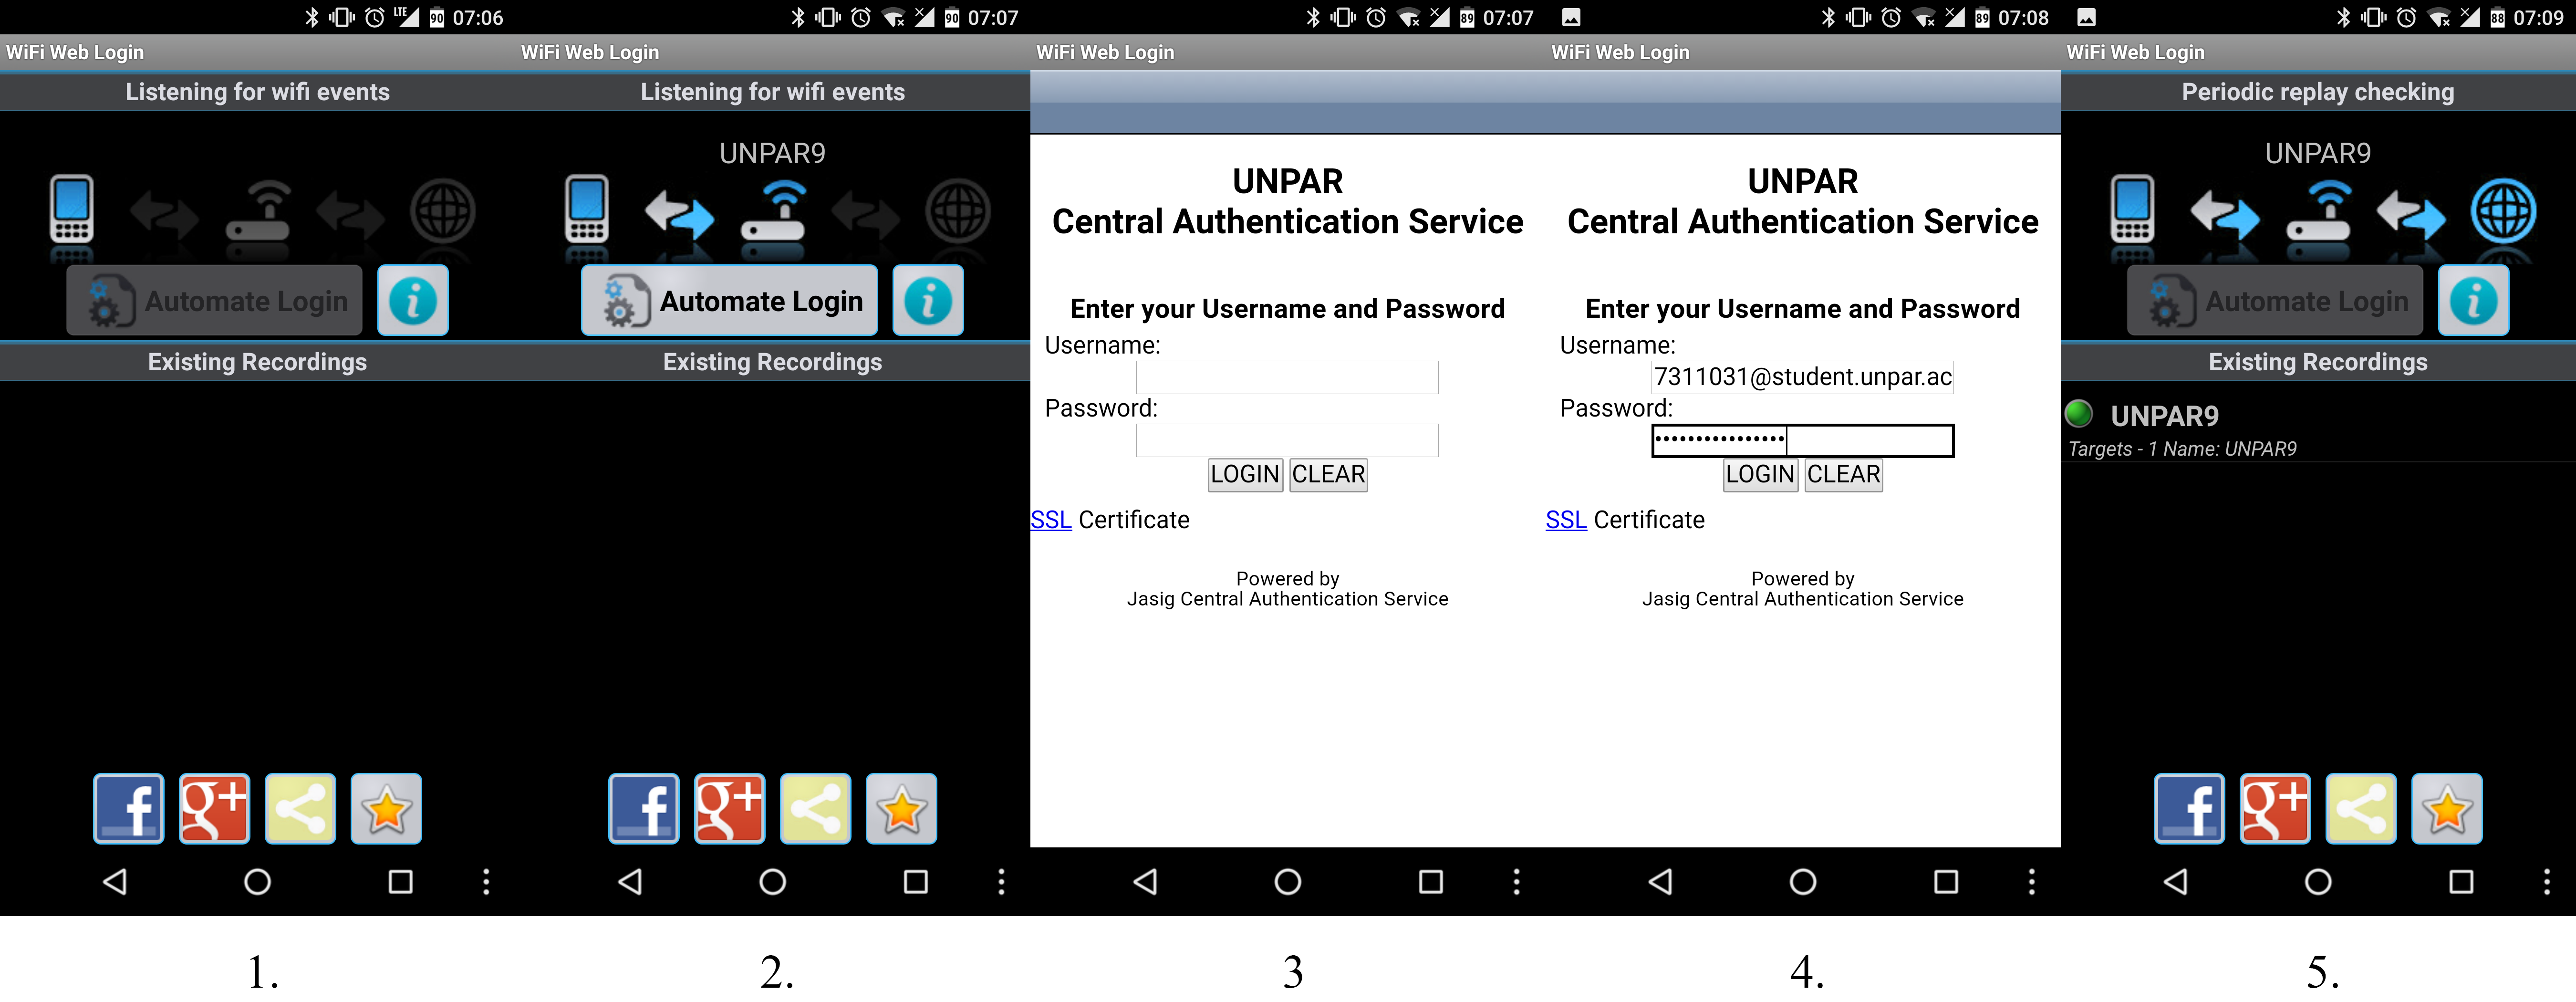
\includegraphics[scale=0.085]{Gambar/screenshot_wifiweblogin.png}
    \caption[Tampilan aplikasi \textit{WiFi Web Login}.]{Tampilan aplikasi \textit{WiFi Web Login}.} 
    \label{fig:screenshot_wifiweblogin}
\end{figure}

Pada gambar \ref{fig:screenshot_wifiweblogin} diperlihatkan langkah-langkah login \textit{captive portal} Unpar sebagai berikut:

\begin{enumerate}
    \item{Menunggu koneksi WiFi.}
    \item{Mendeteksi koneksi WiFi UNPAR9.}
    \item{Menampilkan halaman \textit{captive portal} setelah pengguna menekan tombol \textit{Automate Login}.}
    \item{Pengguna memasukkan username dan password lalu menekan tombol login.}
    \item{Sambungan ke internet terdeteksi dan dilakukan pemeriksaan sambungan berkala.}
\end{enumerate}

\subsubsection{Diagram Alir \textit{WiFi Web Login}}
\label{subsubsec:diagram_alir_wifi_web_login}

Langkah-langkah yang perlu ditempuh oleh aplikasi \textit{WiFi Web Login} dapat digambarkan oleh diagram alir.

\begin{figure}[h]
    \centering
    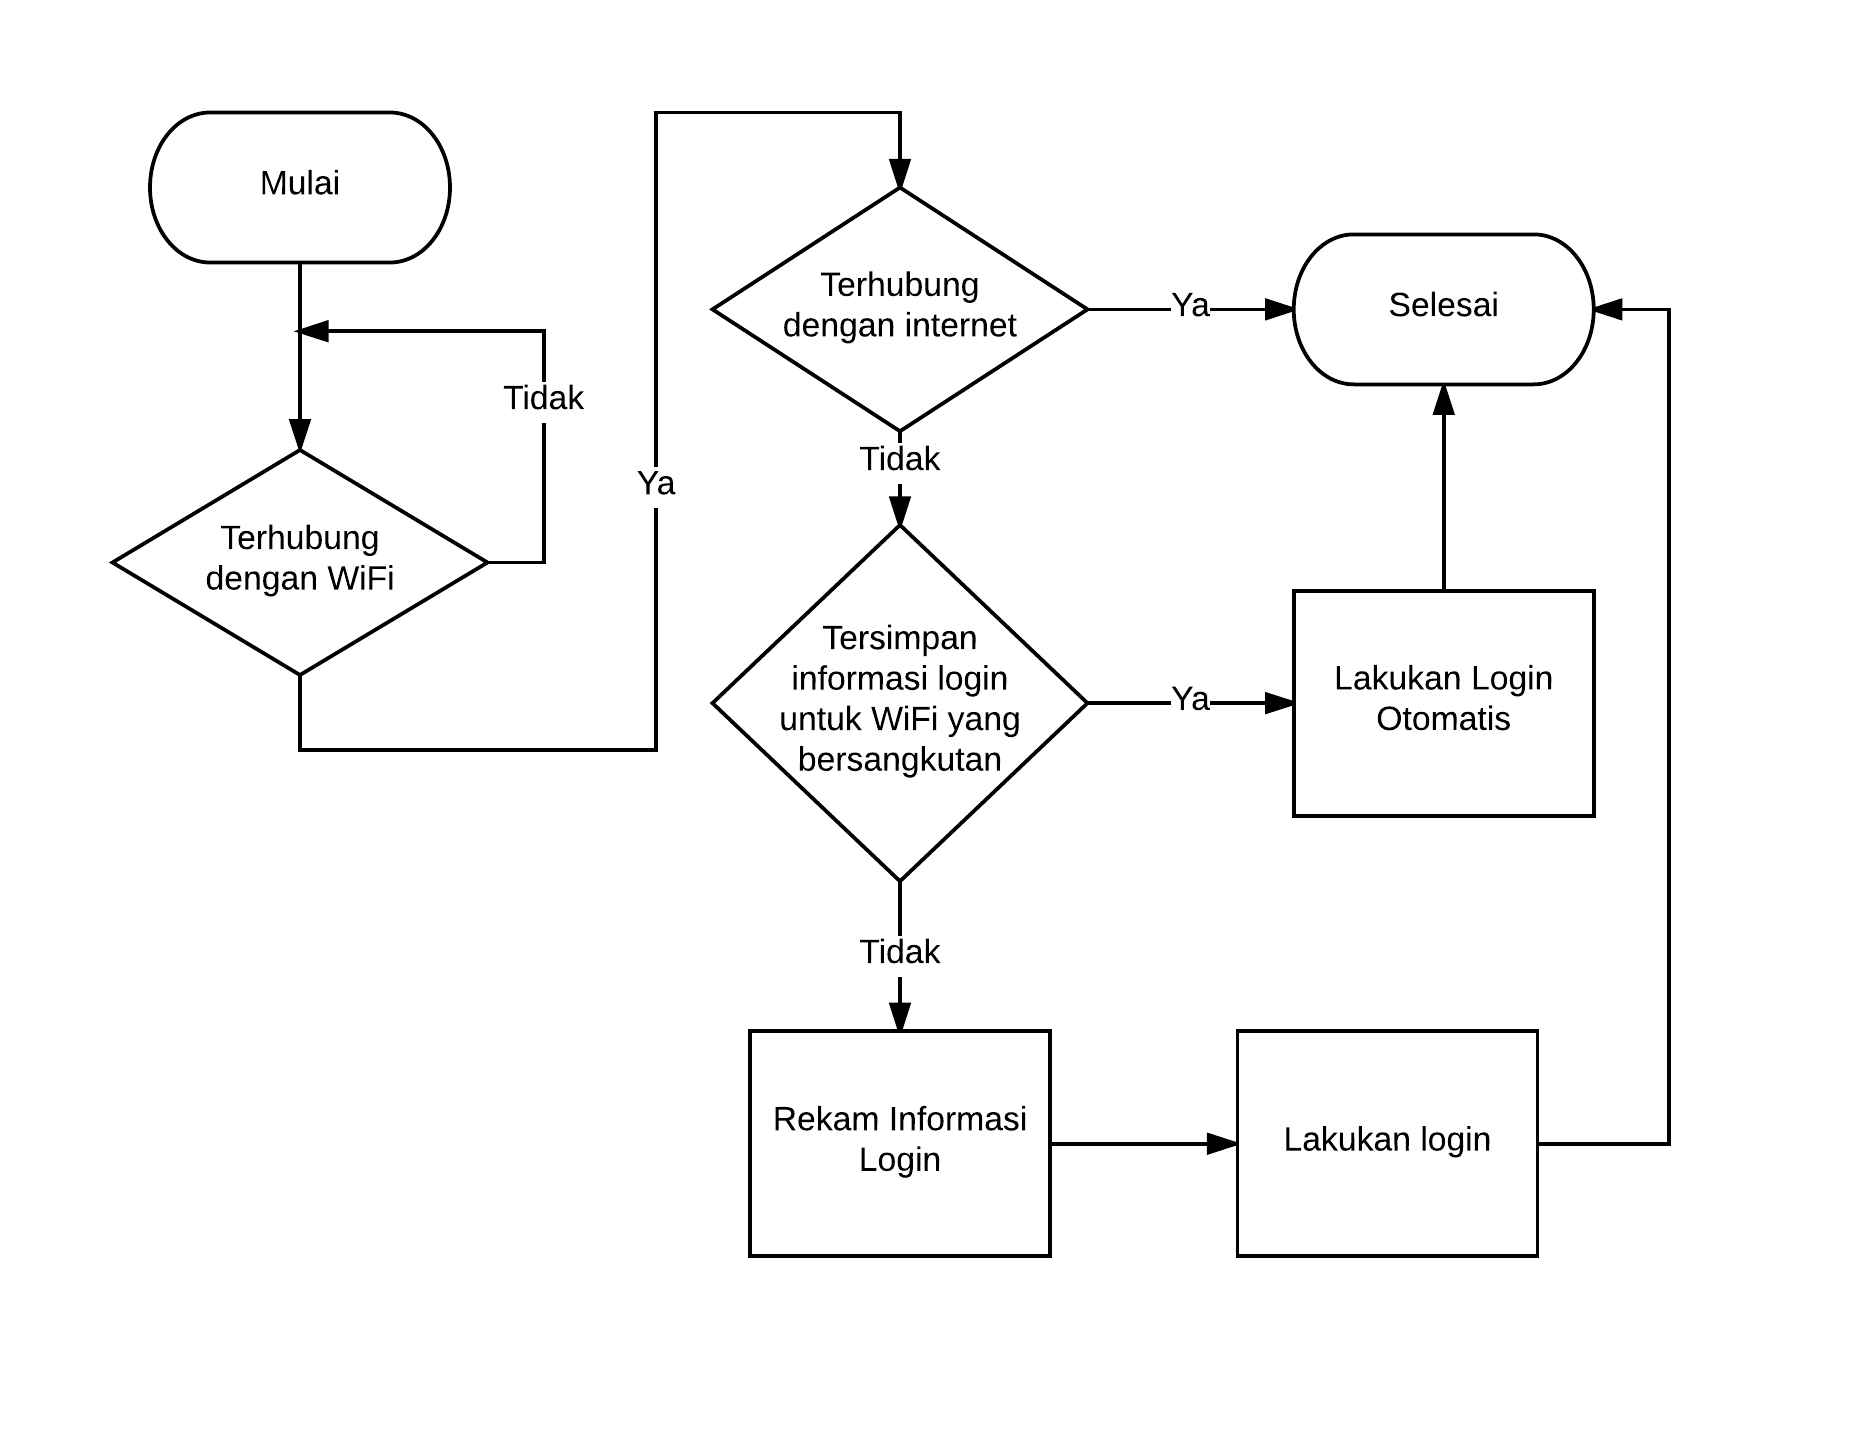
\includegraphics[scale=0.85]{Gambar/WifiWebLogin.png}
    \caption[Diagram alir proses yang perlu dilalui oleh aplikasi \textit{WiFi Web Login}.]{Diagram alir proses yang perlu dilalui oleh aplikasi \textit{WiFi Web Login}.} 
    \label{fig:wifiweblogin}
\end{figure}

Berdasarkan gambar \ref{fig:wifiweblogin}, langkah-langkah yang harus ditempuh untuk melakukan \textit{login} wifi berbasis web pada aplikasi ini adalah:

\begin{enumerate}
    \item{Deteksi sambungan dengan wifi yang bersangkutan.}
    \item{Deteksi hubungan dengan internet.}
    \item{Jika tidak terjadi hubungan dengan internet, deteksi apakah tersimpan informasi login untuk wifi yang bersangkutan.}
    \item{Jika terdapat informasi login untuk wifi yang bersangkutan maka lakukan login otomatis.}
    \item{Jika tidak terdapat informasi login untuk wifi yang bersangkutan maka rekam informasi login dan lakukan login.}
\end{enumerate}

Setelah pengguna melalui sudah pernah melakukan login pertama kali menggunakan aplikasi tersebut, maka aplikasi akan melakukan login otomatis setiap kali terhubung dengan wifi yang bersangkutan.



\section{Analisis Metode Penyimpanan Informasi Login}
\label{sec:metode_penyimpanan}

Penyimpanan informasi login dapat dilakukan dengan beberapa metode, diantaranya adalah dengan menggunakan file teks atau menggunakan PasswordVault. Penyimpanan informasi menggunakan file teks berarti informasi disimpan dalam bentuk \textit{plaintext} dalam file yang diberikan \textit{access permission} tertentu. Sementara itu, penyimpanan informasi menggunakan PasswordVault memanfaatkan kelas API yang terdapat pada \textit{Universal Windows Platform} (UWP).

Informasi yang perlu disimpan untuk dapat melakukan login otomatis adalah \textit{connection fingerprint} (seperti SSID WiFi, url, dan potongan unik dokumen html), username, password, dan langkah-langkah login seperti menekan tombol. Oleh karena itu, metode penyimpanan menggunakan credential locker dan file teks perlu dianalisis untuk dapat ditentukan metode mana yang paling cocok untuk digunakan dalam penelitian ini.

PasswordVault dapat menyimpan informasi yang berisi \textit{resource} (biasanya berupa nama aplikasi atau string unik lainnya), username, dan password. Informasi yang perlu disimpan selain username dan password adalah \textit{connection fingerprint} dan langkah-langkah login. \textit{Connection fingerprint} dapat disimpan pada resource karena sifatnya yang unik. Sementara itu, langkah-langkah login dapat disimpan pada username atau password karena langkah-langkah login dapat disimpan dalam bentuk String. Akan tetapi, langkah-langkah login sebaiknya disimpan pada password, dipisahkan dengan karakter pemisah tertentu, agar username dapat digunakan sebagai \textit{identifier} unik. PasswordVault memiliki batasan 10 kredensial yang dapat disimpan per aplikasi. Jika aplikasi mencoba menyimpan lebih dari 10 kredensial maka akan terjadi exception. Oleh karena hal ini, PasswordVault menjadi pilihan yang kurang baik untuk kebutuhan perangkat lunak pada penelitian ini.

Metode penyimpanan lainnya adalah dengan menggunakan file teks. Penyimpanan informasi mengunakan file teks dapat dilakukan untuk informasi berbasis teks apapun dan tidak ada batasan banyaknya informasi yang dapat disimpan (kecuali batasan perangkat keras seperti kapasitas hard disk). Akan tetapi, file teks dapat dibaca oleh aplikasi manapun, sehingga penyimpanan informasi sensitif tidak dapat dilakukan tanpa adanya metode pengamanan tertentu. Salah satu metode pengamanan yang dapat dilakukan adalah dengan mendeklarasikan \textit{file access permission}. Akan tetapi, karena Windows memiliki \textit{security model} per pengguna dan bukan per aplikasi, maka aplikasi lain yang dijalankan oleh pengguna tersebut memiliki akses yang sama kepada file yang bersangkutan. Metode pengamanan lainnya adalah dengan melakukan enkripsi pada file yang bersangkutan sehingga hanya pemegang kunci yang dapat membaca file tersebut. Enkripsi file pada windows dapat dilakukan menggunakan kelas CryptographicEngine. Kunci enkripsi dan dekripsi dapat disimpan menggunakan PasswordVault atau dengan meminta pengguna untuk memasukkan kunci tersebut setiap kali aplikasi dijalankan.

Metode penyimpanan yang digunakan pada penelitian ini adalah metode penyimpanan menggunakan file teks. Akan tetapi, seperti yang sudah dijabarkan sebelumnya, diperlukan metode pengamanan untuk file teks tersebut. Metode pengamanan yang digunakan adalah enkripsi file teks yang bersangkutan. Kunci enkripsi dan dekripsi dibangun secara random saat aplikasi pertama kali dijalankan dan disimpan menggunakan PasswordVault.



\section{Analisis Metode Rekam dan Kirim Informasi Login}
\label{sec:metode_rekam}

Kelas WebView pada \textit{Universal Windows Platform} (UWP) hanya dapat dihubungkan dengan kode C\# menggunakan javascript. \textit{Method} yang digunakan untuk melakukan eksekusi javascript pada WebView adalah InvokeScriptAsync. Metode ini memiliki parameter string berupa nama fungsi javascript yang ingin dipanggil dan array of string yang berisi argumen yang ingin dikirimkan ke dalam fungsi tersebut. Salah satu fungsi yang dapat dipanggil adalah \textit{eval}. Dengan menggunakan \textit{eval}, ekspresi javascript apapun dapat dijalankan pada WebView. Untuk mengirimkan data dari javascript ke kode C\#, dapat dijalankan fungsi window.external.notify dengan parameter berupa string. Oleh karena itu, diperlukan \textit{encoding} tertentu (seperti JSON\footnote{Singkatan dari JavaScript Object Notation.}) untuk memasukkan lebih dari satu argumen.

InvokeScriptAsync dapat digunakan untuk memanggil fungsi \textit{eval} dengan parameter berupa function yang dapat digunakan untuk menekan tombol atau memasukkan nilai pada \textit{text field} tertentu. Selain itu, dapat dimasukkan event listener yang dapat memanggil window.external.notify menggunakan cara ini. Fungsi window.external.notify dapat membantu mengirimkan event-event seperti mouse click, keypress, atau perubahan nilai pada \textit{text field} yang ada pada halaman HTML pada WebView tersebut.



\section{Analisis Metode Deteksi \textit{Captive Portal}}
\label{sec:deteksi_captive_portal}

\begin{figure}[h]
    \centering
    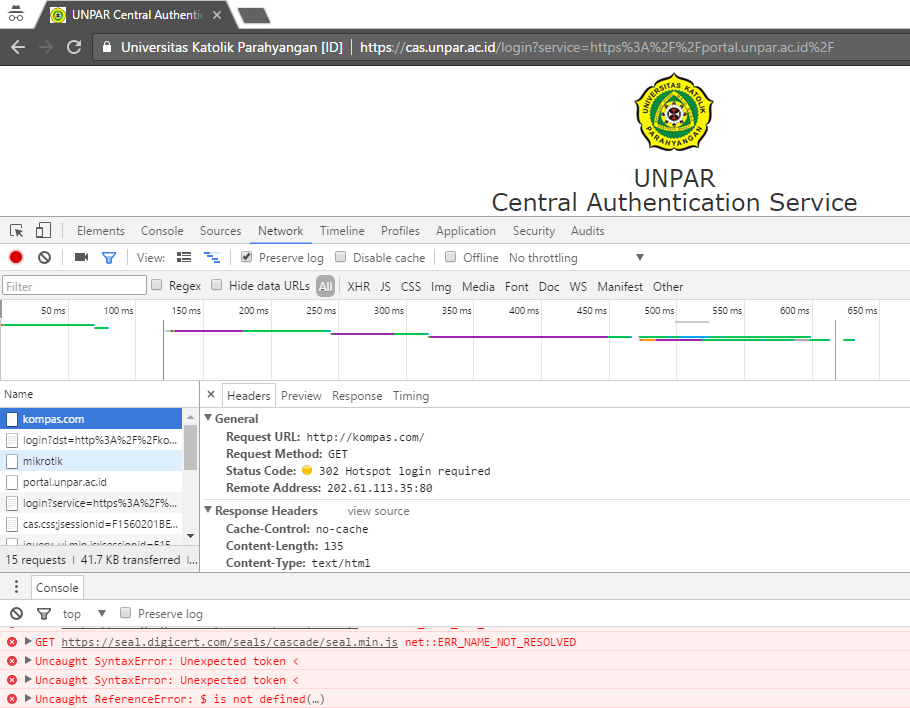
\includegraphics[scale=0.45]{Gambar/Inspect.png}
    \caption[\textit{Screenshot} HTTP \textit{header} yang dikirimkan oleh \textit{captive portal} milik Unpar.]{\textit{Screenshot} HTTP \textit{header} yang dikirimkan oleh \textit{captive portal} milik Unpar.} 
    \label{fig:inspect}
\end{figure}

Berdasarkan teori \textit{captive portal} pada bab 2, dijelaskan bahwa kode status HTTP 511 digunakan untuk memberitahu klien bahwa respon yang didapat bukan berasal dari server tujuan dan diperlukan otentikasi jaringan. Akan tetapi, pada prakteknya, tidak semua \textit{captive portal} melakukan implementasi kode status HTTP 511.

Gambar \ref{fig:inspect} menunjukkan \textit{captive portal} Unpar yang menggunakan kode status HTTP 302 untuk memberitahu klien bahwa diperlukan otentikasi jaringan. Berdasarkan teori mengenai kode status HTTP yang dijabarkan pada bab 2, kode status HTTP 3xx adalah kode status yang menyatakan \textit{redirection}. Oleh karena adanya perbedaan implementasi seperti ini, deteksi \textit{captive portal} menggunakan kode status HTTP tidak dapat dilakukan.

Persamaan implementasi yang dimiliki oleh setiap \textit{captive portal} adalah dibutuhkannya \textit{redirection} yang dapat dikenali oleh \textit{web browser} agar klien selalu diarahkan ke halaman \textit{captive portal} tersebut sebelum melakukan otentikasi. Oleh karena itu, untuk setiap HTTP \textit{request} yang dilakukan oleh klien sebelum melakukan otentikasi, HTTP \textit{response} yang diberikan bukanlah berasal dari server tujuan. Sifat ini dapat dimaanfaatkan untuk keperluan deteksi \textit{captive portal} dengan mengirimkan \textit{request} ke server yang sudah ditentukan sebelumnya, dan mendeteksi apakah \textit{response} yang diberikan sesuai dengan harapan. Jika \textit{response} yang diberikan tidak sesuai dengan harapan, maka dapat diasumsikan bahwa klien dibatasi oleh suatu \textit{captive portal}.

Kelas WebView pada \textit{Universal Windows Platform} (UWP) memiliki kemampuan deteksi \textit{redirection} dan \textit{response} yang tidak sesuai harapan seperti \textit{web browser} pada umumnya. Oleh karena itu, kelas WebView digunakan untuk melakukan deteksi \textit{captive portal} pada penelitian ini tanpa perlu memeriksa kode status HTTP setiap \textit{response}. Penggunaan kelas WebView juga akan mempermudah proses otomatisasi login karena WebView dapat melakukan hal-hal yang dapat dilakukan oleh \textit{web browser} pada umumnya seperti menjalankan javascript dan menampilkan halaman HTML.



\section{Analisis Perangkat Lunak}
\label{sec:analisis_perangkat_lunak}

Bagian ini menjelaskan mengenai diagram \textit{use case} dan diagram kelas perangkat lunak yang dibangun.

\subsection{Diagram Kelas}
\label{sec:diagram_kelas}

Diagram kelas untuk perangkat lunak yang dibangun dapat dilihat pada gambar \ref{fig:diagramkelas}. Seperti pada gambar \ref{fig:diagramkelas}, kelas-kelas yang dibutuhkan pada perangkat lunak ini adalah:

\begin{itemize}
    \item{CaptivePortalDetector\\Kelas ini digunakan untuk mendeteksi keberadaan \textit{captive portal}. Jika captive portal terdeteksi, maka informasi login yang tersimpan dalam Storage digunakan. Jika tidak terdapat informasi login dalam Storage, maka direkam informasi login baru.}
    \item{Storage\\Kelas ini digunakan untuk menyimpan seluruh informasi login dalam bentuk file teks yang sudah terenkripsi.}
    \item{LoginInformation\\Kelas ini digunakan untuk menyimpan informasi login dalam bentuk key atau fingerprint, serta ActionSequence}
    \item{ActionSequence\\Kelas ini digunakan untuk menyimpan langkah-langkah login dalam bentuk urutan aksi dan nilai-nilai yang berkaitan dengan aksi tersebut.}
\end{itemize}

\begin{figure}[h]
    \centering
    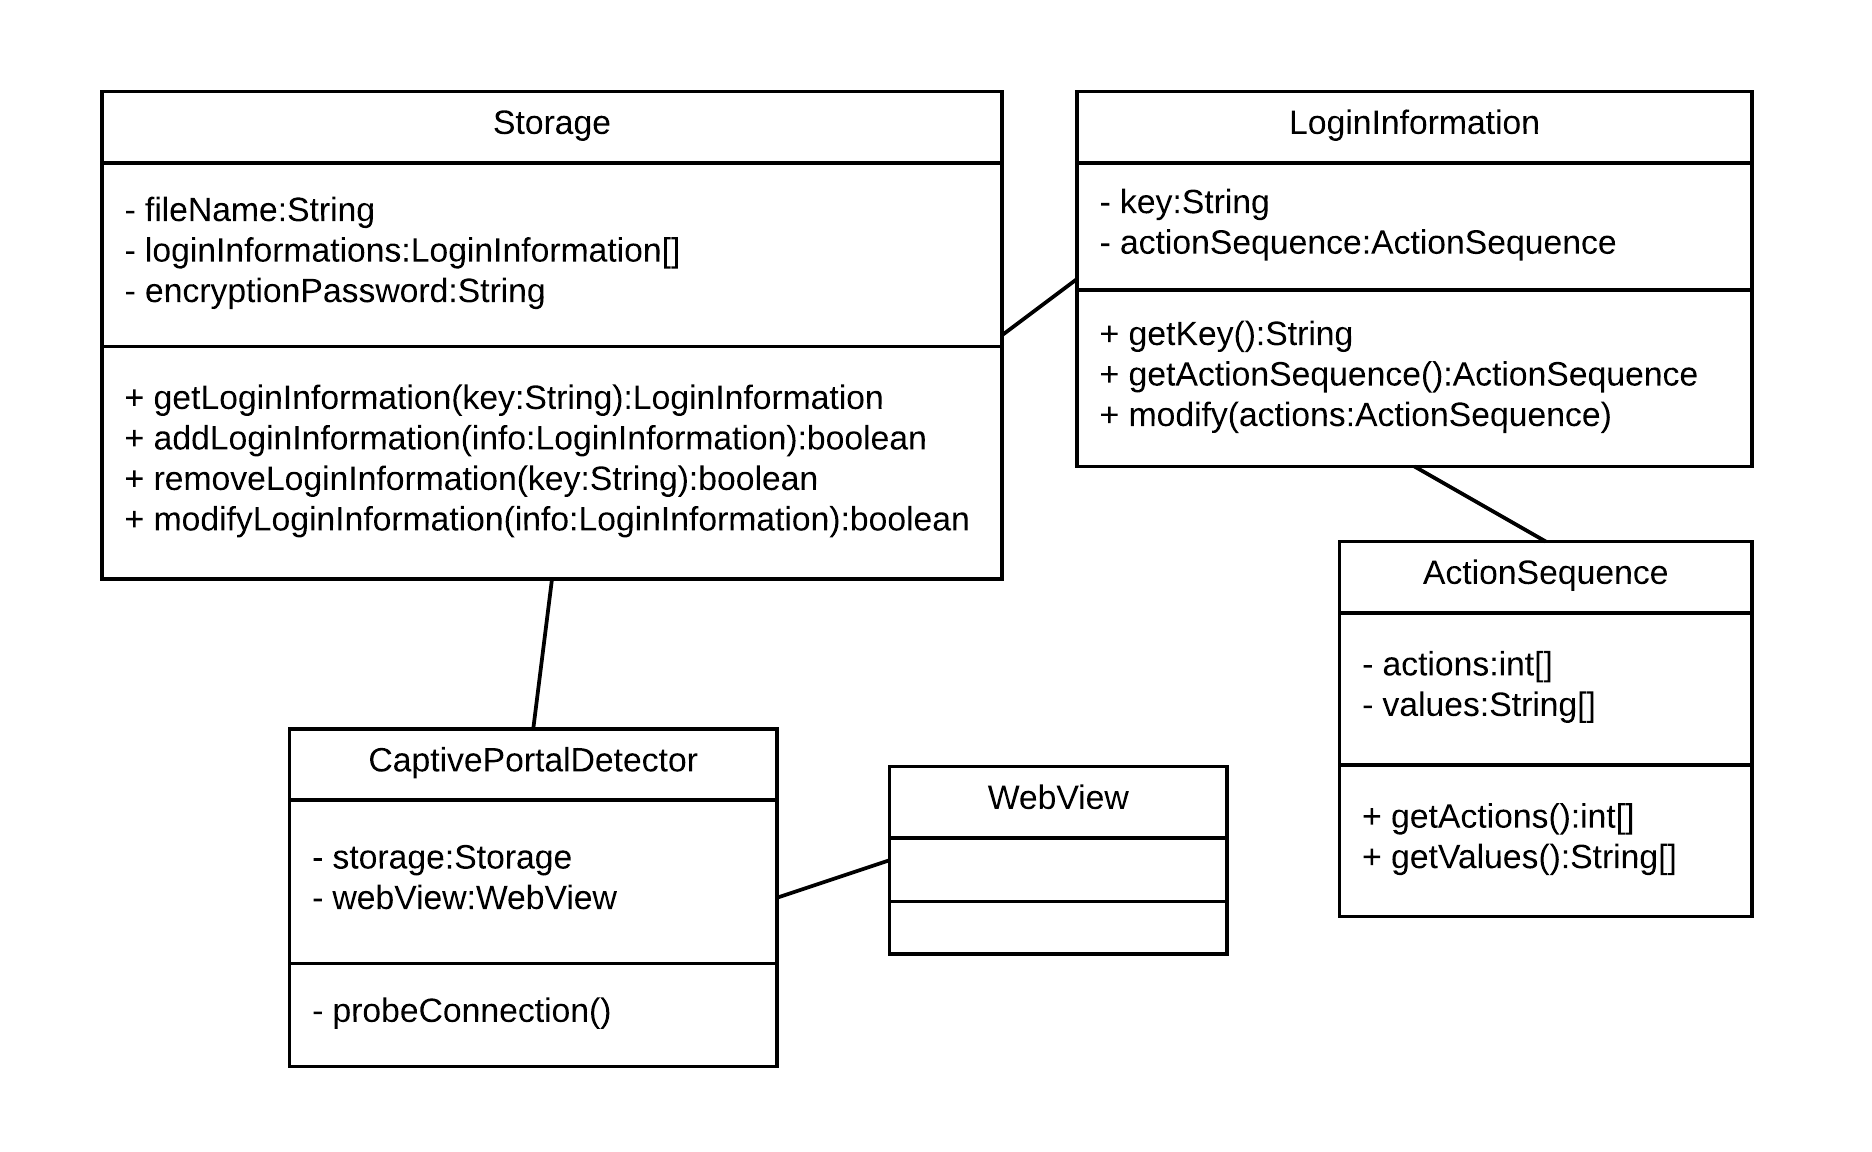
\includegraphics[scale=0.85]{Gambar/classdiagram.png}
    \caption[Diagram kelas untuk perangkat lunak yang dibangun.]{Diagram kelas untuk perangkat lunak yang dibangun.}
    \label{fig:diagramkelas}
\end{figure}

\subsection{Diagram \textit{Use Case}}

Diagram \textit{use case} untuk perangkat lunak yang dibangun dapat dilihat pada gambar \ref{fig:usecase}.

\begin{figure}[h]
    \centering
    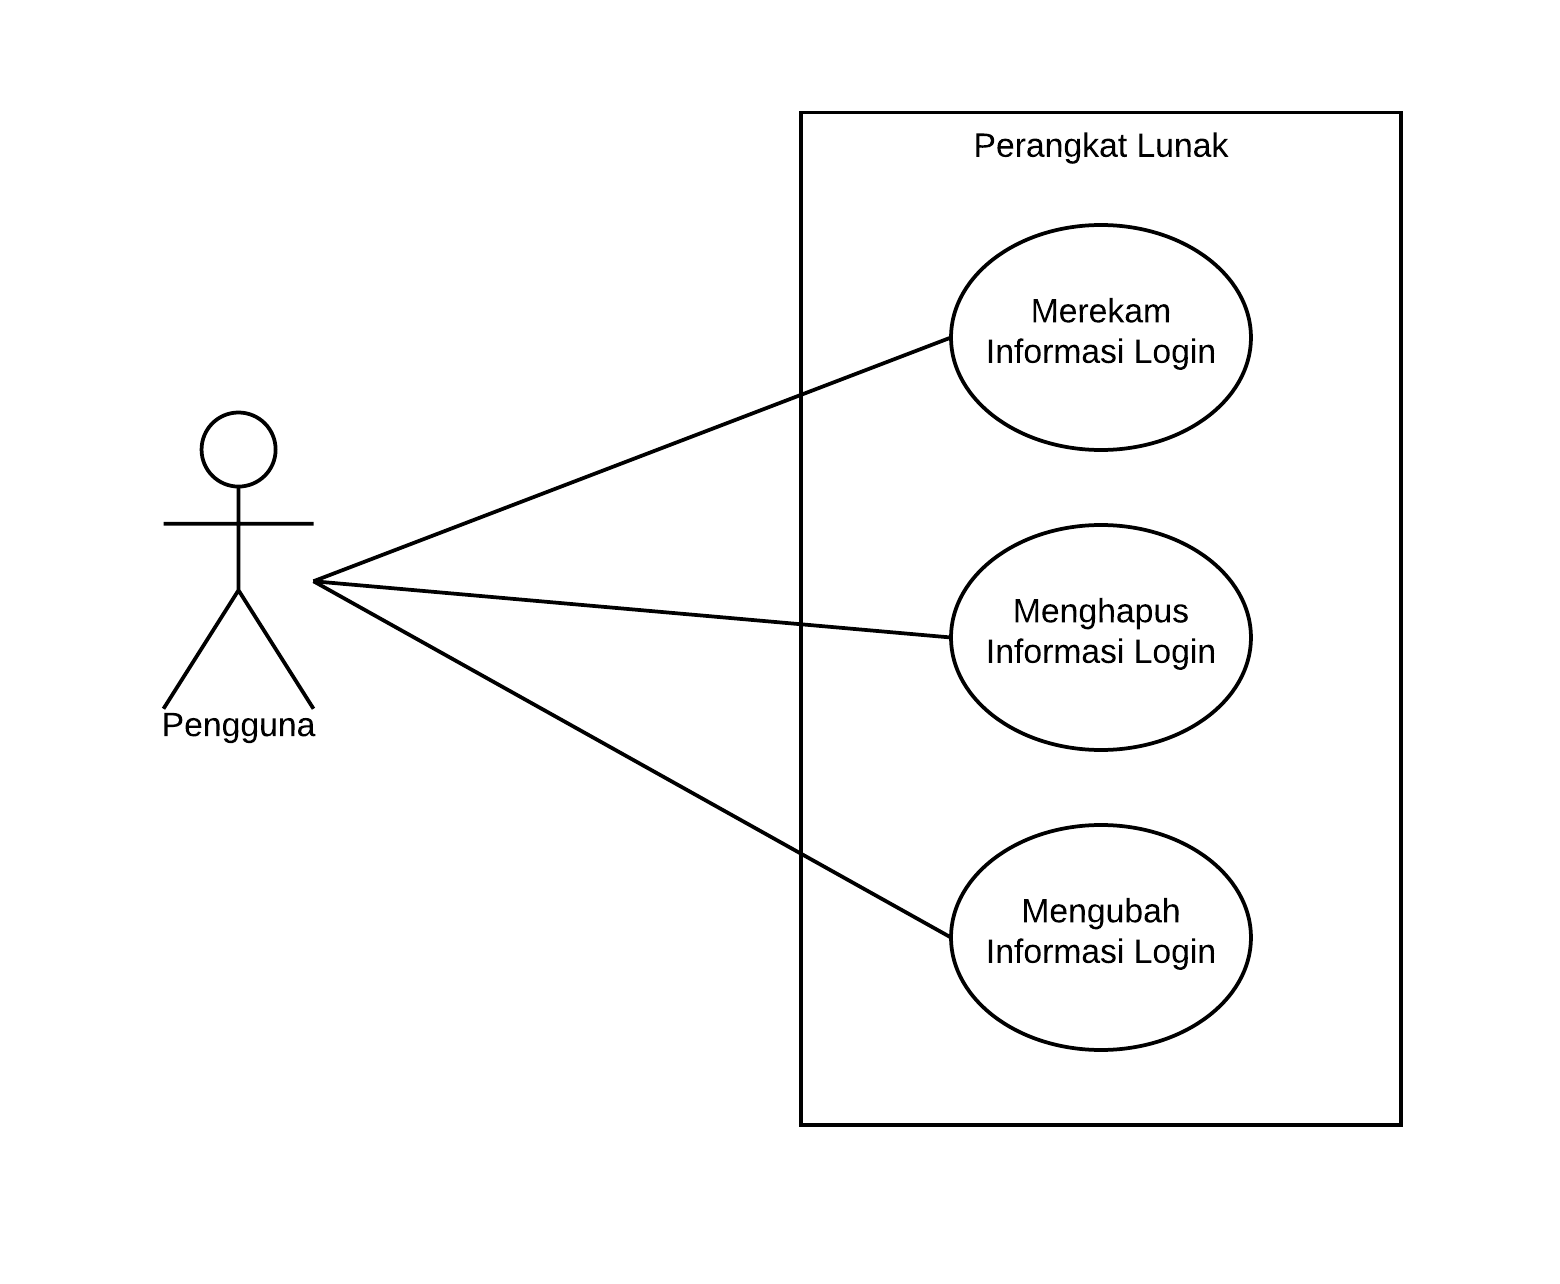
\includegraphics[scale=0.77]{Gambar/usecase.png}
    \caption[Diagram \textit{use case} untuk perangkat lunak yang dibangun.]{Diagram \textit{use case} untuk perangkat lunak yang dibangun.}
    \label{fig:usecase}
\end{figure}

\subsubsection{Skenario merekam informasi login}
Nama: Merekam informasi login\\
Aktor: Pengguna\\
Kondisi awal: Perangkat lunak mendeteksi adanya \textit{captive portal}.\\
Deskripsi: Pengguna menyimpan informasi login.\\
Kondisi Akhir: Informasi login tersimpan di dalam perangkat lunak.\\\\
Skenario:
\begin{enumerate}
    \item{Pengguna memasukkan informasi login ke dalam form HTML.}
    \item{Sistem menyimpan informasi login yang dimasukkan oleh pengguna.}
\end{enumerate}

\subsubsection{Skenario menghapus informasi login}
Nama: Menghapus informasi login\\
Aktor: Pengguna\\
Kondisi awal: Perangkat lunak sudah dijalankan.\\
Deskripsi: Pengguna menghapus informasi login.\\
Kondisi Akhir: Informasi login dihapus dari perangkat lunak.\\\\
Skenario:
\begin{enumerate}
    \item{Pengguna memilih untuk menghapus informasi login.}
    \item{Sistem menghapus informasi login.}
\end{enumerate}

\subsubsection{Skenario mengubah informasi login}
Nama: Mengubah informasi login\\
Aktor: Pengguna\\
Kondisi awal: Perangkat lunak sudah dijalankan.\\
Deskripsi: Pengguna mengubah informasi login.\\
Kondisi Akhir: Informasi login diubah dari perangkat lunak.\\\\
Skenario:
\begin{enumerate}
    \item{Pengguna memilih untuk mengubah informasi login.}
    \item{Sistem menampilkan form ubah informasi login.}
    \item{Pengguna memasukkan informasi login baru.}
    \item{Sistem menghapus informasi login lama dan menyimpan informasi login baru.}
\end{enumerate}

\subsubsection{Skenario memicu login otomatis}
Nama: Memicu login otomatis\\
Aktor: WiFi\\
Kondisi awal: Perangkat lunak sudah dijalankan.\\
Deskripsi: Sistem memicu login otomatis berdasarkan perubahan status WiFi.\\
Kondisi Akhir: Klien terotentikasi pada \textit{captive portal}.\\\\
Skenario:
\begin{enumerate}
    \item{Sistem mendeteksi adanya koneksi WiFi yang terjadi.}
    \item{Sistem mendeteksi adanya \textit{captive portal}.}
    \item{Sistem mendeteksi adanya informasi login untuk \textit{captive portal} tersebut.}
    \item{Sistem mengirimkan informasi login kepada \textit{captive portal}.}
    \item{Sistem mendeteksi koneksi dengan internet dan klien sudah terotentikasi pada \textit{captive portal} tersebut.}
\end{enumerate}